\section{Nombre: Chara enana}   \label{per:chara}
\subsection{Descripción:}
Ave mágica que habita el Mictlán. Su cuerpo de presenta ligeras llagas de donde salen estalagmitas, estas llagas se pueden ver principalmente en su espalada y cráneo. Su plumaje es de color azul oscuro. 
\subsection{Status:}
\begin{itemize}
	\item Enemigo normal.
\end{itemize}
\subsection{Imagen}

%\begin{figure}
%	\centering
%	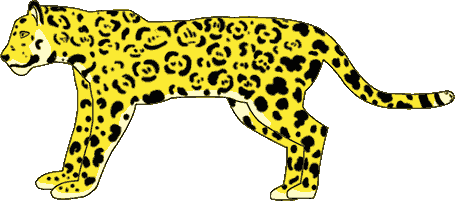
\includegraphics[height=0.2 \textheight]{Imagenes/jaguar}
%	\caption{Jaguar.}
%	\label{fig:jaguar}
%\end{figure}
\subsection{Encuentro:}
En el nivel 5 (ver apartado \ref{Nivel:Niv05}).
\subsection{Habilidades:}
\begin{itemize}
	\item Vuelo en picada (ver apartado \ref{hab.Vpicada}).
\end{itemize}
\subsection{Patrón de ataque:}
Su movimiento se da en dos puntos horizontales: A y B. Realiza un patrullaje de punto A al B y del B al A, cada vez que regresa a alguno de los puntos por segunda vez consecutiva ejecuta la habilidad de vuelo en picada (ver apartado \ref{hab.Vpicada}).
\subsection{Bloques de animación:}
	\begin{itemize}
		\item Animación vuelo.
		\item Animación caída en picada.
	\end{itemize}